% $Id$

\chapter{The Translation Process}
The system can be activated with a sequence of
commands of the following form, typically embedded within a script.

\begin{verbatim}
       latex      x            (or `tex x')
       latex      x
       latex      x
       tex4ht     x
       t4ht       x
\end{verbatim}


The three compilations with \latex (or \tex) are needed to ensure
proper links.  The approach is illustrated in the following picture.

\ifhtml
 \Tg<img src="figure.png"/>
\else
 \begin{center}
  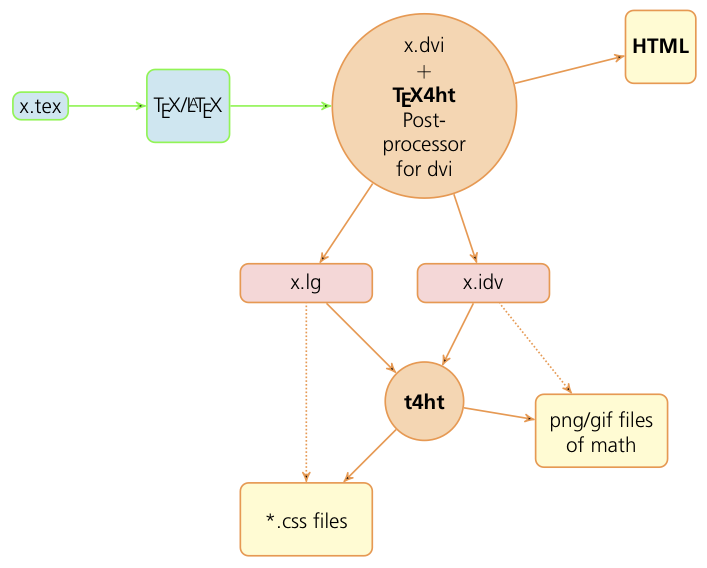
\includegraphics{figure.png}
 \end{center}
\fi

\begin{itemize}
\item \texttt{x.tex}: This is a source \tex or \latex or other \tex file
  that imports the style files \verb'tex4ht.sty' and \verb'*.4ht'.  The
  style files define the features for the output.

\item \texttt{tex4ht}: The output of \tex is a standard verb+dvi+ file
  interleaved with special instructions for the postprocessor
  \verb'tex4ht' to use.  The special instructions come from implicit and
  explicit requests made in the source file through commands of
  \texht.

  The utility \verb'tex4ht' translates the \verb+dvi+ code into
  standard text, while obeying the requests it gets from the special
  instructions. The special instructions may request the creation of
  files, insertion of \html code, filtering of pictures, and so forth.

  In the extreme case that the source code contains no commands of
  \texht, \verb+tex4ht+ gets pure \verb+dvi+ code and it outputs
  (almost) plain text with no hypertext elements in it.

  The special (\verb+\special+) instructions seeded in the verb+dvi+
  code are not understood by verb+dvi+ processors other than those of
  \texht.

\item \texttt{x.idv}: This is a \verb+dvi+ file extracted from
  \verb'x.dvi', and it contains the pictures needed in the \html
  files.

\item \texttt{x.lg}: This is a log file listing the pictures of
  \verb+x.idv+, the png files that should be created, \textsm{CSS}
  information, and user directives introduced through the
  \verb+\Needs{...}+ command.

\item \texttt{t4ht}: This is an interpreter for executing the requests
  made in the \verb'x.lg' script.

\end{itemize}

